\documentclass{article}
\usepackage[utf8]{inputenc}
\usepackage{amsmath}
\usepackage{graphicx}
\usepackage[procnames]{listings}
\usepackage{color}
\usepackage{indentfirst}
\usepackage{xcolor}
\usepackage{sectsty}
\usepackage[explicit]{titlesec}


\usepackage[normalem]{ulem}

%\title{Library Information System\\ System Requirement Specification}

%\author{}
%\date{March 2016}

\begin{document}

%\maketitle

\section{INTRODUCTION}

\subsection{Purpose}
This Software Requirement Specification (SRS) document provides a complete list and description of all the functions and specifications of the Library Information System (LIS).

The software is meant to hold the records of the books and the users and to provide the functionality of issuing and returning books. Apart from that the users can also request to reserve a required book if available in the library.

The expected audience of this document are Library clerk , librarian of an institute and the developer of the software.

\subsection{Document Conventions}
The conventions used in the document are given as follows
\begin{itemize}
\item 
\end{itemize}
\subsection{Intended Audience}
The intended readers of this document are the developers of the software, testers, library owners
and managers and coordinators.
Any suggested changes on the requirements listed on this document should be included in
the last version of it so it can be a reference to developing and validating teams.
\subsection{Scope}
LIS is a GUI tool that enahnces the manual process of keeping records in a library.This is an appication which has been designed keeping in mind that it is meant to run on Library computers and to allow the library to keep a track of the books present.It allows the users to check availabilty whenever they want. It also allows the users to reserve a book in advance if needed. The librarian is able to keep a record of the overdue books, add new books, dispose old data, add new member or delete a member. 

It is a powerful but still functionally simple library management software for big libraries and can provide a free easy-to-use system for rising libraries.

Presently the maximum number of books has been kept constant to ensure a fruitful implementation of the software architecture. In future the list of books may be made to increase dynamically to make it more realistic.
\subsection{References}
The following references have been consulted to make a suitable and effective software for library information system.

\begin{itemize}
\item IEEE standard 830-1998 recommended practice for Software Requirements Specifications-Description
\item 
\end{itemize}


\section{OVERALL DESCRIPTION}
\subsection{Product Perspective}

\subsection{Product Features}
The product provides the features to create a librarian , library clerks and a set of users comprising of UG student, PG student, Faculty and Research Scholar.

All the users irrespective of their type can issue and return a book.The librarian has some special functions like creation of a library member/user. The librarian can have access to account of any user and can look into it in case need arises.
Library clerks on the other hand can add and remove a book from the database of the library. They also have been assigned methods to impose fine in case of defautlters.

Finally there is a non-physical member called as LIS (syatem admin) which is autonomous and monitors all the finctioning of the software. It automatically notifies about the delays to the clerks and helps to update and keep track of all the activities of the software.

A class diagram showing the relationship is given below to enhance the understanding of the workflow.
\\
\\
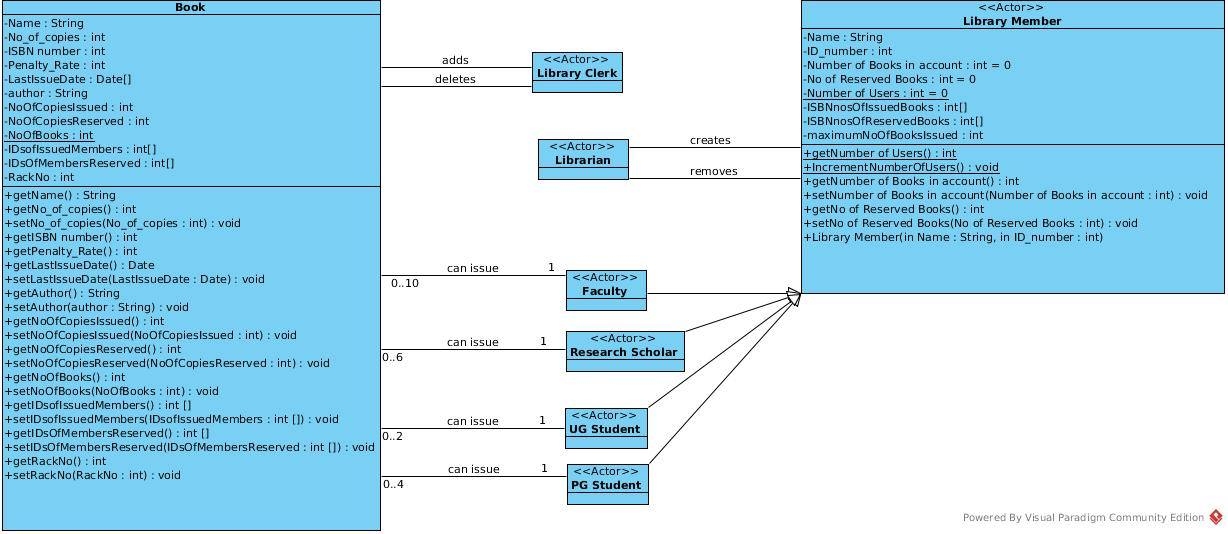
\includegraphics[scale=0.25]{images/classDiagram}

\subsection{User Classes and Characteristics}

\subsection{Operating Environment}
The software is designed to run on the following environments :
\begin{itemize}
\item Windows 
\item Ubuntu 14.04.03 (LTS version)

Any OS with the support of Java JDK and JRE libraries 1.7 and above can be used to execute the software.
\end{itemize}

\subsection{Design and Implementation Constraints}
This software is optimized to run on a maximum of 10000 books .
Exceeding this number can result in a slower running time of the algorithm and thus the execution may not fruitful enough.

\subsection{User Documentation}
User manual $:$

\subsection{Assumptions and Dependencies}


\section{SYSTEM FEATURES}
\subsection{System Feature 1}

\section{EXTERNAL INTERAFCE REQUIREMENTS}
\subsection{User Interfaces}
\subsection{Hardware Interfaces}
\begin{enumerate}
\item The software is run offline so hard disk with sufficient space of about --- is required to store and save the records for further use
\item Keyboard and mouse to interact with the GUI
\end{enumerate}
\subsection{Software Interfaces}
\begin{enumerate}
\item Back end  $:$ Built using Java and DBMS
\item Front end $:$ Using Java 
\end{enumerate}

\subsection{Communication Interfaces}

\section{OTHER NONFUNCTIONAL REQUIREMENTS}
\subsection{Performance Requirements}
With the Library Information System the librarian and library clerk can process a book transaction in a faster speed .
The members will be able to check the status of the checked out items and can also borrow and return a book in a short amount of time.
Automatic updates in the account of each user will enable them to know about the item they have cjecked out and all the relevant details due to which they do not need to consult or ask the library clerk each time.
The background system admin will automatically perform the above mentioned updation in the accounts in the background autonomously without explicit invocation.
In case of defaulters the fine and other penalties should be automatically reported and saved in the record once the deadline has crossed . This is also performed by the syatem admin (referred as LIS itself) in the background.
ALl the background tasks should not compromise with the UX of the software.All the background processes should be methodically handled and not affect the runtime functionalities of the software

\subsection{Safety Requirements}
Only the valid users can change the records that too only in their respective account.
\subsection{Security Requirements}
The sytem must be highly secure in the login part.
No user should be able to access a domain outside his reach.
Care must be taken to keep the user accounts secure and all the book transaction should be properly updated to the corresponding user.

\subsection{Software Quality Requirements}


\subsubsection{Reliability requirements}
The background database should always be updated so that whenever a member visits he/she can get the latest information required.
\subsubsection{Usability Requirements}
The software must be user-friendly so that the user can easily perform all the tasks which the software is meant to do.It must have a soothing UX design and clear instructions to guide the user.
\\In case of any error suitable error messages must be displayed to assist the user.


\section{OTHER REQUIREMENTS}
\end{document}